\begin{figure}
\begin{fullpage}
\begin{center}
    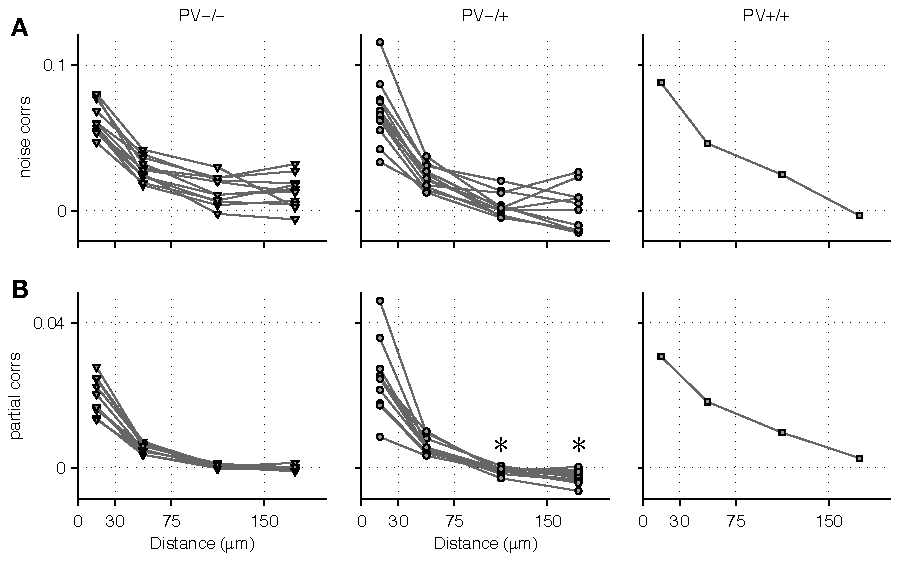
\includegraphics[width=\textwidth]{./figures/pv-fig3.pdf}
\end{center}
\caption[Distance dependence of functional connectivity by cell pair type]
{{\bf Distance dependence of functional connectivity by cell pair type}

{\bf A.} Average noise correlations binned by distance in 11 sites for PV--/-- cell pairs (left), PV--/+ cell pairs (middle), and PV+/+ cell pairs (right, pooled from  all sites).  

{\bf B.} Average regularized partial noise correlations binned by distance in 11 sites for PV--/-- cell pairs (left), PV--/+ cell pairs (middle), and PV+/+ cell pairs (right, pooled from  all sites).  The differentiation between cell pair types is stronger for partial correlations than noise correlations. For PV--/+ pairs, the average partial correlations were negative (p<0.005, signed rank test) for intersomatic distances greater than 75 $\mu$m.  In contrast, the partial correlations for PV--/-- cell pairs dropped to zero in the same range.

}\label{fig:pv3}
\end{fullpage}
\end{figure}
